\documentclass[letterpaper,12pt]{article}
\setlength{\headheight}{14.49998pt}
\usepackage{fancyhdr}
\usepackage{lipsum,graphicx}
\usepackage{amsmath, amsfonts, amssymb, ragged2e}
\usepackage{amsthm}
\usepackage{bookmark}
\usepackage{listings}
\usepackage{times}
\usepackage{color}
\title{Summary for CPEN 212}
\author{Tom Wang}
\date{Spring 2024}

\fancypagestyle{plain}{
    \fancyhf{}
    \fancyhead[L]{Tom Wang}
    \fancyhead[R]{\thepage}
}

\begin{document}
\maketitle
\section{Calling conventions}
In assembly, sometimes we need to make system calls to the OS. We need to
follow the calling conventions to make sure that the OS can understand our
request.

\subsection{Start with examples}
Start we an example: \begin{lstlisting}
    .text
    .global _start
_start:
    mov x0, 42
    mov x8, 93
    svc 0
\end{lstlisting}
Here, we are trying to make a system call to exit the program. We need to put
the system call number in x8, and the argument in x0. The system call number
for exit is 93. We then use svc 0 to make the system call.

\begin{itemize}
    \item $.text$ tells the assembler/linker that code follows.
    \item $.global$ tells the assembler/linker that the symbol \_start is visible to the linker. This is the entry point of the program.
    \item Then we put the value in x0 and x8. Here x0 is the argument for the system
          call, and x8 is the system call number.
\end{itemize}

To compile this and run (on Linux/arm64): \begin{lstlisting}
    as -o foo.o foo.s
    ld -o foo foo.o
    ./foo
    echo \$?
\end{lstlisting}
The last line prints the exit code of the program. In this case, it should be
42.
\begin{itemize}
    \item $as$ is the assembler. It takes the assembly code and produces an object file.
    \item $ld$ is the linker. It takes the object file and produces an executable.
    \item $./foo$ runs the executable.
    \item $echo \$?$ prints the exit code of the program.
\end{itemize}

Another example: \begin{lstlisting}
    .text
    .global _start
_start:
    mov x8, 64
    mov x0, 1
    adr x1, txt 
    mov x2, len 
    svc 0
    mov x8, 93
    mov x0, 42
    svc 0
txt: .ascii "goodbye, cruel world!\n"
len = . - txt
\end{lstlisting}
This program prints "goodbye, cruel world!" and exits with code 42. Here, we
are using the write system call. The system call number for write is 64. The
arguments are: \begin{itemize}
    \item system call number 64 in x8 means write
    \item file descriptor 1 in x0 means stdout, which is the standard output.
    \item address of the string in x1
    \item length of the string in x2
    \item system call number 93 in x8 means exit
    \item exit code 42 in x0
    \item system call 0 to make the system call
    \item the string to print
    \item The length is calculated by subtracting the address of the string from the
          current location. (note that in the stack, the address grows downwards)
\end{itemize}

One more example: \begin{lstlisting}
length:
    mov x2, -1
length_rec:
    add x2, x2, 1
    ldrb w1, [x0], 1
    cbnz w1, length_rec
    mov x0, x2
    ret


.global _start
_start:
    adr x0, txt
    bl length
    mov x2, x0
    mov x0, 1
    adr x1, txt
    mov x8, 64
    svc 0
    mov x8, 93
    mov x0, 0
    svc 0
txt: .asciz "goodbye, cruel world!\textbackslash n"


    //Here we decompose bl and ret
    str lr, [sp, -4]! //store the lr original value
    mov lr, [pc, 4] 
    //load the address of the next instruction
    mov pc, length //jump to the function
    ...\dots
    //now returning
    mov pc, lr //return to the address in lr
    ldr lr, [sp] //restore the lr value
    add sp, sp, 4 //restore the stack pointer
    //that is it
    
\end{lstlisting}
Here instead of using the length variable, we are using a function to calculate
the length of the string. The function is called length. It takes the address
of the string as the argument and returns the length of the string in x0. The
function is called using bl, which is a branch and link. It branches to the
function and saves the address of the next instruction in the link register.
The function returns using ret, which branches to the address in the link
register.

Explain code line by line:\begin{itemize}
    \item $mov x2, -1$ sets x2 to -1. This is the initial value of the length.
    \item $add x2, x2, 1$ increments x2 by 1. Increase the length by 1 for each loop.
    \item $ldrb w1, [x0], 1$ loads a byte from the address in x0 into w1. The address in x0 is then incremented by 1. This loads the next character in the string. If we want to increment by 1 then load, we can use $ldrb w1, [x0, 1]!$. The $!$ means increment after.
    \item $cbnz w1, length_rec$ checks if w1 is not zero. If it is not zero, then it branches to length\_rec. This is the loop condition. If the character is not zero, then we continue the loop.
    \item $mov x0, x2$ moves the length in x2 to x0. This is the return value.
    \item $ret$ returns to the address in the link register.
    \item The rest is the same as before.
\end{itemize}

\subsection{calling convention}
Calling convention is not enforced by hardware, but it is a convention to make
sure that the caller and callee agree on how to pass arguments and return
values.

The caller is the function that calls another function. The callee is the
function that is called. The calling convention is a contract between the
caller and the callee. The caller must follow the calling convention to call
the callee. The callee must follow the calling convention to be called by the
caller. The calling convention includes:

Here are some rules:
\begin{itemize}
    \item bl is for address relative to the current instruction. b is for absolute
          address. blr is for register relative to the current instruction. br is for
          absolute register.
    \item function arguments are passed in registers x0-x7. If there are more than 8
          arguments, then the rest are passed on the stack.
    \item function results are in x0. If there are more, we use x1 to x7 then the stack.
          x8 is used for system call number.
    \item return address is in lr (x30). lr is the link register. It is used to store the
          return address when we call a function. It is also used to store the address of
          the next instruction when we use bl.
    \item Caller is responsible for saving registers x0-x18. The callee can use them
          without saving them. The callee is responsible for saving registers x19-x30.
          The caller can use them without saving them.
    \item The stack grows downwards. The stack pointer is in x31. The stack pointer
          points to the last item in the stack. The stack pointer is decremented when we
          push something onto the stack. The stack pointer is incremented when we pop
          something from the stack.
\end{itemize}
\subsection{call frame}
The call frame is the part of the stack that is used to store information about
the function call. It includes the return address, the saved registers, and the
local variables.

The call frame is created when we call a function. It is destroyed when the
function returns. The call frame is created by the caller. The caller is
responsible for saving the registers and creating the local variables. The
callee is responsible for saving the return address.

Usually we have stack pointer which points to the last item in the stack.

We also have frame pointer which points to the start of the call frame. The
frame pointer is used to access the local variables.

The frame pointer is not necessary, but it makes it easier to access the local
variables.

But if we have dynamically sized stack allocation (memory allocation
functions), then fp is obligatory.

\subsection{Jumping to a function}
To jump to a function, we use bl. bl is a branch and link.

It branches to the function and saves the address of the next instruction in
the link register. The function returns using ret, which branches to the
address in the link register.

Back in the time when there is no bl, we have to do this manually. We have to
save the return address in the stack, then jump to the function. The function
then returns by popping the return address from the stack and jumping to it.

Another way is to specify the line of return when creating the callee function.
And then when we call a function, the caller will write the return address to
the specified line. And then the callee will jump to that line when it returns.
This is called a trampoline. Not to nice to use, but it is a way to do it back
in the day.

\subsection{ABI}
ABI is the application binary interface. It is a standard for binary
interfaces. It specifies the calling convention, the system call numbers, and
the system call arguments. It is used to make sure that the caller and callee
agree on how to pass arguments and return values.

\subsubsection{stack-based ABI}
\begin{itemize}
    \item stacks are sequential. If we spawn two functions, the stack must grow into two
          different directions. how to achieve this? We can use two different stacks.
    \item stack spaces are deallocated on return, so we can reuse the stack space.
\end{itemize}
\section{Haxx}
Start with a C example: \begin{lstlisting}[language=C]
    int main() {
        volatile long ans = 42;
        char buf[16];
        gets(buf);
        //latex does not support printf properly
        printf(ans);
        return 0;
    }
    
\end{lstlisting}
gets() reads a line from stdin into the buffer pointed to by s until either a
terminating newline or EOF, which it replaces with a null byte ('\textbackslash
0'). No check for buffer overrun is performed (see BUGS below).

So this program is vulnerable to buffer overflow. We can overflow the buffer
and overwrite the value of ans.
\subsection{Analysis of the victim}
By observing, volatile makes sure that ans lies on the stack. Then we allocated
16 bytes for buf (char is 1 byte each). Now the pointer of buf is 16 bytes away
from ans. With that, have a look at the compiled assembly code:
\begin{lstlisting}
main:
    stp x29, x30, [sp, -48]!
    mov x29, sp
    mov x0, 42
    str x0, [x29, 40]
    add x0, x29, 24
    bl gets
    ... rest of the code 
\end{lstlisting}
stp is store pair. It stores two registers in the stack. The first register x29
(Stack pointer, pointing to the top of the stack of the parent function) is
stored at the address in sp. The second register x30 (Link register, parent
function address) is stored at the address in sp minus 8. The stack pointer is
then decremented by 48. So 48 lines of memory is allocated for the call frame.

Then x29 keeps the current program sp. x0 is loaded with 42. Then x0 is stored
in the address in x29 plus 40. So the address of ans is x29 plus 40 which is
the bottom of the frame (Stack grows downwards, so right next to the parent
function's top of stack). Then x0 is loaded with x29 plus 24. So x0 is loaded
with the address of buf. Then we call gets.

\includegraphics*{./Images/Haxx victim stack.jpg}

Now if we input more than 16 bytes, we can overflow the buffer and overwrite
the value of ans.

For example, we can input ``ffffffff ffffffff 3905''. This will overwrite the
value of ans with 3905.

\subsection{Typical attack pattern}
\begin{itemize}
    \item Find a program running on target (maybe as root)
    \item scan binary for potential buffer overflows. E.g, look for gets, strcpy, strcat,
          sprintf, etc.
    \item craft input that will overflow the buffer and overwrite something interesting
    \item objective: execute arbitrary code
\end{itemize}
\subsubsection{Jump to arbitrary code}
In ARMv8, typically, we save lr to the top of the stack before bl to another
function.

Since overwrite in this case writes to the higher address, but lr for the
current call frame is at the lower address, we can't overwrite the current
function's lr.

But we can overwrite the return address of the parent function which will lie
just above the bottom of the call frame. So we can overwrite the return address
of the parent function with the address of the code we want to execute. Then
when the parent function returns, it will jump to the code we want to execute.

\subsection{Code injection}
Now we know how to jump to other addresses, but we still need to inject our
code into the program. How do we pass arguments to the code you want to
execute?

One way to do it is to overwrite the stack with the machine code that
corresponds to the assembly code you want to execute. Then you can pass
arguments to the code by putting them in the stack.

\includegraphics*[scale = 0.6]{./Images/Haxx attack v3.jpg}

Note that the ARM64 code is little-endian. So the first byte is the least
significant byte. We put the code to overwrite the space for buf and ans. The
value printed is the third line of ARM machine code in large-endian.

we overwrite the lr with the start of the ARM code address ``00 00 ff ff ff ff
ee b8''. So the pc will jump to your written code.

Also, since ARM only allows 16-bit constant input, we can load 16 bits of a
register at a time. That is why we have to load the value of ans into x0 and x1
separately by shifting the constant input.

Now last line ``br x1'' would allow us to jump to the address in x1. The
argument we want to pass has its address in x0, which is the last line we
overwritten.

\subsubsection{Code injection limitations}
\begin{itemize}
    \item stack/heap often non-executable.\begin{itemize}
              \item enforced by virtual memory system (Segmentation fault)
              \item It will crash the program if we try to execute code in the stack or heap.
          \end{itemize}
    \item stack/heap locations often randomized (ASLR) \begin{itemize}
              \item enforced by the virtual memory system
              \item It will randomize the location of the stack and heap. So we can't predict the
                    location of the stack or heap.
          \end{itemize}
\end{itemize}

\subsection{Gadgets}
Gadgets are small pieces of code that end with a return instruction.

Since code injection is not executable, we can find some existing code
(gadgets) and chain them together to do what we want. It could be either in the
program itself or in a library.

\subsubsection{return-oriented programming (ROP)}
\begin{enumerate}
    \item find gadgets in the program or libraries
    \item put the address of the gadget in the stack by overflowing the buffer
    \item prepare the arguments for the gadget by overflowing the buffer
    \item construct a chain of gadgets that does what you want
\end{enumerate}
Depending on the found gadgets, we inject the useful value into the stack by overflowing the buffer. The ultimate goal is to change the value of the link register and pass the desired arguments to the gadget.

Refer to mie's slides for examples.
\subsubsection{more advanced ROP}
\begin{itemize}
    \item can be any indirect jump instruction, not just ret. For example \begin{lstlisting}
        ldp x1, x2, [sp], 16
        br x2
    \end{lstlisting}
    \item can overwrite virtual function pointers in C++ objects.
    \item SROP: play with signals to set all registers.
\end{itemize}

\subsection{Non-executable stack/data}
For most systems, the stack and data are non-executable.

Virtual memory system enforces this. It will crash the program if we try to
execute code in the stack or heap. Also called $W^X$ policy (write xor
execute).

However, we can use ROP to make a system call to make the stack executable.
Then we can inject our code into the stack and execute it.

\subsection{Address space layout randomization (ASLR)}
ASLR randomizes the location of the stack and heap. So we can't predict the
location of the stack or heap.

Virtual memory system enforces this. It will randomize the location of the
stack and heap. So we can't predict the location of the stack or heap.

\subsubsection{Limitations of ASLR}
\begin{itemize}
    \item not all bits are random, it is possible to brute-force the address space. Just
          need more trials.
    \item Library locations are not randomized since programs need to find libraries to
          use them once the program starts. So we can use gadgets in libraries.
    \item Programs on machines like servers are not restarted often. So we can use
          brute-force to find the address of the stack and heap.
\end{itemize}
\subsection{Array bounds checking}
Some programming languages like Java and Python have array bounds checking. It
checks if the index is inside the bounds for each operation. So we can't
overflow the buffer.

This prevents writing to memory that we don't own. However, for languages that
could do pointer arithmetic, we can still do buffer overflow. C and C++ are
typical examples.

Also, people sometimes disable array bounds checking for performance reasons.
This kind of fast but unsafe code is hackers' best friend.

\subsection{Stack canaries}
\begin{itemize}
    \item put some value on the stack below the return address (or frame pointer if it
          exists)
    \item check the value, see if it is modified before ret.
    \item if modified, abort the program. Might print something like ``stack smashing
          detected'' (Should work just like an exception)
    \item the variants can be 0, random, or random XOR with the return address.
\end{itemize}
However, there are still limitations to it:\begin{itemize}
    \item if exception handling is hacked, we can still bypass the stack canaries.
    \item the pattern can only detect \textbf{some} overflows.
    \item fixed canary value can be easily discovered.
    \item canary value can still be leaked.
    \item canary feature is usually not enabled by default.
\end{itemize}
\subsection{safe(r) programming languages}
\begin{itemize}
    \item Java, Python, etc. have array bounds checking.
    \item Rust, Go, etc. have memory safety.
    \item C/C++ are still the most popular language.
    \item safe languages are not always safe. For example, Java has a lot of
          vulnerabilities.
    \item Some languages guarantee safety via \textbf{type system}. For example, Rust. It
          is checked by the compiler at compile time. However, only guaranteed if used
          properly. Also, these languages are not as popular as C/C++.
\end{itemize}
\section{Memory management}
\includegraphics*{./Images/Memory of a process.png}

Each process has its own memory space. The memory space is divided into
segments. The segments are: \begin{itemize}
    \item text segment: the code of the program
    \item data segment: the variables
    \item heap: the dynamic memory allocation
    \item stack: the local variables and the call frames
\end{itemize}
Heap and stack grow towards each other. The stack grows downwards. The heap grows upwards.

\begin{itemize}
    \item Stack is easy to allocate but disappears after the function returns.
    \item Heap is harder to allocate but can be used after the function returns.
\end{itemize}

\subsection{Allocation strategies}
\begin{itemize}
    \item automated: \begin{itemize}
              \item garbage collection: the memory is automatically deallocated when it is no
                    longer used. It is used in languages like Java and Python.
              \item reference counting: the memory is automatically deallocated when the reference
                    the count is zero. It is used in languages like C++. (There are limitations to
                    this, for example, circular references)
              \item Hard to implement but easy to use
          \end{itemize}
    \item manual: allocate and deallocate pairs. \begin{itemize}
              \item malloc()+free() or new()+delete() comes in pairs. (It is a contract that must
                    be obeyed)
              \item easy to implement but hard to use. (lots of bugs)
          \end{itemize}
\end{itemize}
\subsection{Memory allocation}
\begin{itemize}
    \item want high utilization and low fragmentation\begin{itemize}
              \item physical memory is limited among all processes
              \item OS only gives big chunks of memory to processes (usually 4KB pages)
              \item most allocs are small, few words to a few KB
          \end{itemize}
    \item want high allocation throughput. Minimize the management overhead.
\end{itemize}

Recall the stack allocation:\begin{itemize}
    \item to allocate, just move the stack pointer downwards
    \item to deallocate, just move the stack pointer upwards
    \item easy to implement and efficient
    \item However it does not support dynamic allocation which does not work for heap.
\end{itemize}
\subsubsection{Challenges}
\begin{itemize}
    \item how to keep track of block size?
    \item how to keep track of free blocks?
    \item how to find a free block?
    \item how to allocate a block? which free block to use?
\end{itemize}
\subsubsection{tracking allocation size}
For each block, we can store the size of the block which can be used to find
the start and the end of the current block. Thus we can find the neighboring
blocks.

Note that the blocks can also request the size of both neighboring blocks. Just
having the size at the start of the block is not enough. We need the size at
both the end and the start of the block.

\includegraphics*{./Images/Memory track size.png}

Note that we may or may not contain the padding there to follow the alignment
rules of the system. At the same time, we can omit the lower bits of the size
to store the status of the block since size should always occupy the whole line
in the system no matter what the system is working with. Lastly, the a there
can indicate the status of the block. 1 means allocated, 0 means free.
\subsubsection{finding a free block}
let $p$ = heap start: for each block $b$ at $p$:\begin{itemize}
    \item if $b$ is free \textbf{and} $b$ is big enough, return $b$
    \item else $p$ = $p$ + size of $b$
    \item keep going until the end of the heap \begin{itemize}
              \item either we find a free block
              \item or we run out of memory
              \item or ask OS for more memory
          \end{itemize}
\end{itemize}
This is a ``first fit'' strategy. It is simple and fast, but it can lead to fragmentation.

We can have ``next fit'' as well:\begin{itemize}
    \item keep track of the last block we allocated, return the next free and big enough
          block after that
    \item can be faster than first fit
    \item but still can lead to fragmentation (even worse than first fit)
\end{itemize}

Also we can have ``best fit'':\begin{itemize}
    \item return the smallest free block that is big enough
    \item but it is slow (overhead of searching for the smallest block)
\end{itemize}
\subsubsection{coalescing and boundary tags}
\includegraphics*[scale = 0.7]{./Images/Coalescing.png}

As shown in the figure, if we just free the 4-byte block, we will have two free
blocks connecting together which we can merge by coalescing. This is done by
checking the status of the neighboring blocks. If they are free, we can merge
them together. This is called coalescing.

Note that we can use either the header or the boundary tag to track the
neighboring blocks. So it does not matter if the free neighboring block is at
the higher address or the lower address. We can always find it by checking the
status and the size of the neighboring blocks.

In some cases, we might need to connect both neighboring blocks together if it
happens that they are both free.
\subsection{explicit freelist}
The above section is an example of an implicit freelist. The freelist is
implicit because it is not explicitly stored. It is stored in the heap itself.
We need to find them by checking the status of the neighboring blocks.

We can also have an explicit freelist. We can have a linked list of free
blocks. Each free block contains a pointer to the next free block. This is
called an explicit freelist because the freelist is explicitly stored in the
heap.

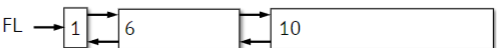
\includegraphics{Images/Doble-linked explicit freelist.png}
\subsubsection{data structure}
For a double-linked list, we can have a pointer to the next free block and a
pointer to the previous free block. This is called a doubly linked list. It is
useful when we want to remove a block from the list. We can just change the
pointers of the previous and the next block to remove the current block from
the list.

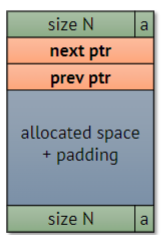
\includegraphics{Images/explicit freelist data structure.png}

This way, we can find the free block by just following the pointers. We can
also remove the block from the list by changing the pointers. We can also add a
block to the list by changing the pointers.
\subsubsection{Coalescing}
Note that coalescing is not achieved by the explicit freelist since it does not
know the neighboring blocks. We need to use the implicit freelist to coalesce
the blocks. So we still need to header and footer to track the neighboring
blocks.

\subsubsection{Optimizing boundary tags}
Consider when we use the boundary tags? We use it when we want to coalesce the
blocks. So we can optimize the boundary tags by only using it when we want to
coalesce the blocks which would only happen for the free blocks.

To know if the previous block is free, we use another bit in the header to
indicate if the previous block is free. Note that lower bits of size can be
omitted because of alignment with bytes reason.

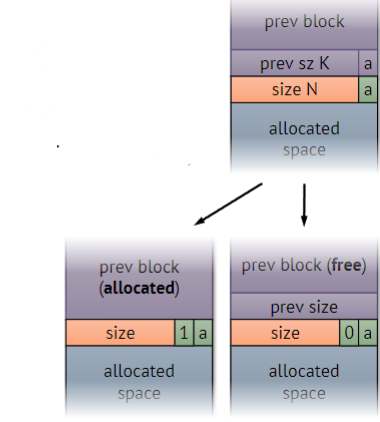
\includegraphics{Images/Optimizing boundary tags.png}
\subsection{segregated free lists}
If we mix all sizes of free blocks in one list, then it becomes hard to track
the sizes and find the best one to use and do coalescing.

It is better to keep a list for some special size of blocks. Usually, $2^k$
bytes or Fibonacci bytes. The reason for choosing these two is that they add up
to each other, making them easy to do coalesce.

\subsubsection{buddy allocator}
\begin{itemize}
    \item what if one FL is empty? Just steal another block from the FL with larger sizes
          and break it into two.
    \item what if we coaleasce? Just put the coalesced block into the FL with larger
          sizes.
\end{itemize}
\subsubsection{slab allocator}
\begin{itemize}
    \item what if common sizes are not powers of 2? Fro example, we use size of 3 all the
          time. Then we waste internal fragmentation overhead of 25\%.
    \item We can fix it by using slab allocator. We can allocate a slab of memory and
          divide it into blocks of the same size. Then we can use the blocks to allocate
          memory. For example, we have so many size 3 right? Just pick a 256 block and
          break them to allocate size 3. Overhead is only $\frac{255}{256}=0.4$\%.
\end{itemize}
\section{Garbage collection}
To automatically free the memory that is no longer used. It is used in
languages like Java and Python.

Explore a few ways to achieve it:
\subsection{Delete upon destruction}
When variables go out of scope, the destructor is called. Why don't we just
free the memory there?
\begin{lstlisting}[language=C++]
    template <typename T> class ptr{
        T* p;
        public:
        //some other code:
        virtual ~ptr() {delete p;}
        //upon destruction, delete the memory
    }
    void foo() {
        auto c = ptr<complex>(new complex(1,2));
        //do something with c
        //c is destroyed upon exiting foo()
    }
    void foo1() {
        auto c = ptr<complex>(new complex(1,2));
        bar(c);
        //some other use of pointers
    }
    void bar(ptr<complex> c) {
        //do something with c
        //c is destroyed upon exiting bar()
    }
\end{lstlisting}
Note that it works well with foo(), however, it can cause trouble with foo1().
The reason is that we can't free the memory until we exit foo1(). But we have
already deleted it upon exiting bar(). So we can't use it anymore.

So we need a better way of doing it.
\subsection{Reference counting}
Why don't we just count the number of references to the memory? When the number
of references is zero, we can free the memory.
\begin{itemize}
    \item upon initialization, set the reference count to 1
    \item upon assignment, increment the reference count of the new pointer and decrement
          the reference count of the old pointer
    \item upon destruction, decrement the reference count and free the memory if the
          reference count is zero
\end{itemize}
Note that we store the number inside the memory itself instead of the pointers. This is because if we store it in the pointers, for each update, we need to update all of the pointers to keep them present. This is not efficient.
\subsubsection{Overhead}
\begin{itemize}
    \item Space overhead: each smart memory has a reference count. Then smart pointers
          have two pointers, one to the memory and one to the reference count.
    \item Performance overhead: each access is just 1 pointer dereference. However, each
          copy/destroy is 1 pointer dereference and 1 arithmetic operation.
\end{itemize}
\subsubsection{Limitations}
circular references: if two objects refer to each other, then the reference
count will never reach zero.

\includegraphics*[scale = 0.6]{./Images/Circular Reference.jpg}

In the picture there, it is possible that we lost the reference to the memory
while the reference count is not zero. This is a memory leak.
\subsection{reachability}
So the real problem is reachability. If the memory is not reachable, then we
can free it. So we need to find a way to check if the memory is reachable.

Observation: once a memory is not reachable, it will never be reachable again.
So we can free it.

Now we need to know how to check if the memory is reachable. We can use a graph
to represent the memory. Each node is a memory block. Each edge is a reference
from one block to another. Then we can use graph traversal to check if the
memory is reachable.
\subsubsection{A tracing garbage collector}
\begin{itemize}
    \item start from the roots (global variables, local variables, etc.)
    \item follow the references to other memory blocks
    \item mark the memory blocks as reachable
    \item free the memory blocks that are not marked
\end{itemize}
\subsubsection{The tri-colour abstraction}
\begin{itemize}
    \item white: not visited
    \item grey: visited but not finished (A data that contains multiple references to
          other data, and we did not visit all of them)
    \item black: visited and finished
\end{itemize}
Using this abstraction, we can use some graph algorithms to do the garbage collection. In the end, all the block that we mark as white can be freed.
\subsubsection{mark and sweep}
\begin{itemize}
    \item pause the program
    \item traverse the graph from the roots
    \item mark the reachable memory blocks
    \item sweep the memory blocks that are not marked
    \item resume the program
\end{itemize}
\subsubsection{mark and sweep implementation}
\begin{itemize}
    \item Note that we need a bit in the memory to indicate if the memory is marked. We
          can just steal another bit from the size. Since we already have one for
          allocation status and one for the previous block, it requires it to be 8-byte
          aligned. So we can just steal the lower bit of the size to indicate if the
          memory is marked. A negligible overhead.
    \item We also need to distinguish between pointers and integers. We can use the lower
          bit of the pointer to indicate if it is a pointer or an integer.

          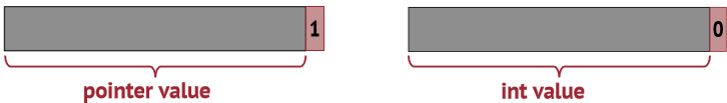
\includegraphics[scale = 0.6]{./Images/Pointer and Integer distinguishing.png}

          Note that we chose integers to be even numbers. This is to make sure that
          pointer arithmetics with integers keep the lower bit to be 1 which keeps
          consistency with the pointers.

          drawback of this approach is the smaller range of integers.

          Note that this might not be a problem in some programming languages where the
          data structure makes clear of where the pointers are. Java and Python are
          examples of this.
    \item Backtracking during traversal: the current way of doing it would store all the
          pointers as we mark, which will take up a lot of memory space. However, by the
          time we are doing the garbage collection, we are close to running out of
          memory, which could be a problem.

          One of the way to solve it is by reversing the pointers. We use a temprory
          pointer to store the current branch and reverse the visiting node to point to
          the parent node. This way we can always trace back to the parent node without
          storing all the pointers.

          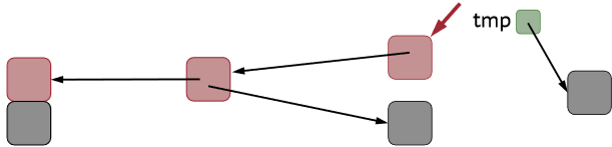
\includegraphics[scale = 0.6]{Images/BackTracking.png}

          Refer to Miezko's slides for an animation of this process.

          This approach only takes $O(1)$ space. However, it is slower than the previous
          approach and it stops the program for a longer time since pointers are moved,
          the program cannot visit all the nodes in progress. No \textbf{concurrent}
          garbage collection.
\end{itemize}
\subsection{Stop and Copy}
Mark and sweep is nice, but it creates fragmentation. Free space is \textbf{not
    contiguous}.

Stop and copy is a way to solve this problem. It is a two-space collector. It
has two spaces: from-space and to-space. It copies the reachable memory blocks
from from-space to to-space. Then it swaps the two spaces.

Refer to Miezko's slides for an animation of this process.

\begin{itemize}
    \item Stop and Copy would require us to only use half of the memory space. This is a
          big overhead. But it is not that bad. Most of the time, the objects we left in
          the heap does not live for too long. So a much more frequent garbage collection
          is not that bad given that we get huge chunk of free space instead of
          fragmented space.
    \item It is \textbf{Not Concurrent}. It stops the program since it moves the
          pointers.
    \item Note the use of two pointers \textbf{scan} and \textbf{free}. \begin{itemize}
              \item scan: if all pointers inside the node are visited, and the pointed blocks are
                    moved to the to-space, then we can move the pointer to the next node. We paint
                    the node black following the tri-colour abstraction.
              \item free: if the node is reachable. Paint the node grey if so and move on.
          \end{itemize}
\end{itemize}
\subsection{refcount vs mark and sweep s stop and copy}
\includegraphics*[scale=0.7]{Images/refcount vs mark and sweep s stop and copy.png}
\subsection{mark and compact}
Wonder if there is a way to use the entire heap nad still avoid fragmentation
(compact)?

Idea: save the working pointers somewhere else so that we can use the whole
sapce. \begin{itemize}
    \item keep an extra space to store them.
    \item keep the pointers in the heap itself as a break table and move it accordingly
          if needed.
\end{itemize}
Refer to miezko's slides for an animation of this process.

\subsection{ephemeral garbage collection}
Observation: most allocs have short lifetimes. Why not just garbage collect the
young objects?

Split heap into generations:\begin{itemize}
    \item young generation (nursery): for new objects
    \item when the young generation is full, garbage collects it
    \item if an object survives a few garbage collections, move it to the old generation
    \item we can have multiple levels of generations, apply gc as well if they are full
\end{itemize}
Note that gc is fast if we keep the young generation (nursery) small.
\subsection{Weak references}
\begin{itemize}
    \item a weak reference is a reference that does not prevent the object from being
          garbage collected
    \item it is useful for caches, observers, etc.
    \item The object is reachable, but the event is not happening anymore. So we can free
          the memory.
    \item it is used in languages like Java and Python
\end{itemize}
\subsection{non-deterministic finalization}
\begin{itemize}
    \item finalization is the process of freeing the memory
    \item For example, in C++, the destructor is called when the object goes out of
          scope, and sockets and locks in Java and Python are closed when the object is
          garbage-collected
    \item it is non-deterministic because we don't know when the memory will be freed
\end{itemize}
\subsection{Conservative garbage collection}
Some languages do not distinguish between pointers and integers. They can also
do pointer arithmetics with pointers.

We can use some logic to find the difference, for example, small numbers are
generally not pointers. However, this is not always true. If not pointing
inside blocks, then it is not a heap pointer.

These tricks are not always reliable. So we can use conservative garbage
collection. It is a way to do garbage collection without knowing the exact
location of the pointers. We can just assume that the integers are pointers and
do garbage collection.
\section{Virtual memory}
Virtual memory is needed since we want to run multiple instances simultaneously
and use the same memory addresses.

Each program would think that they have the entire memory to itself.
\subsection{Virtual memory abstraction}
\begin{itemize}
    \item each program has its own virtual memory space
    \item the virtual memory space is divided into pages
    \item the pages are mapped to physical memory
    \item the mapping is done by the operating system
\end{itemize}
In a 64-bit architecture, we usually divide into 4KB pages. Thus the last 12 bits of a Virtual Address is the offset of the page. The rest of the bits are the page numbers.

\subsubsection{levels of page tables}
Page tables can be divided into levels.

\begin{itemize}
    \item PT0: 47-39
    \item PT1: 38-30
    \item PT2: 29-21
    \item PT3: 20-12
    \item offset: 11-0
\end{itemize}
Each cell in $PT_i$ is a pointer to the next level $PT_{i+1}$, which is a new page. The last level is the physical memory.

Each entry of the page table contains the physical address of the next level
page table. The actual data page is stored in the last level, accessed by the
offset which contains bytes.
\subsection{PTE (Page Table Entry)}
There are lots of other bits in the entry of the virtual page table to indicate
something else:\begin{itemize}
    \item valid bit: if the page is valid (if it is not valid, then it is not in the
          physical memory)
    \item dirty bit: if the page is modified (if it is modified, then we need to write it
          back to the disk when we swap it out)
    \item read-only bit: if the page is read-only (if it is read-only, then we can't
          write to it)
    \item user-accessible bit: if the page is accessible by the user (if it is not
          accessible, then we can't access it)
    \item non-executable bit: if the page is non-executable (if it is non-executable,
          then we can't execute code in it)
    \item physical page number: the address of the page in the physical memory
    \item recently used bit: if the page is used recently (if it is used recently, then
          we can keep it in the physical memory, otherwise, it becomes a candidate for
          swapping out)
\end{itemize}
If there is insufficient permission, then we will get a segmentation fault.
\subsection{VM uses}
\subsubsection{more memory}
We have limited physical memory. We can use virtual memory to use the disk as
memory. We can swap the pages in and out of the physical memory. This is called
paging.

Upon more memory requests, we either terminate some programs to free up the RAM
or move some pages to the disk to free up the RAM.

Use the idea of \textbf{locality} to make use of the physical memory. We can
use the pages that are used recently and the pages that are used together.

\subsubsection{Page fault}
When we access a page that is not in the physical memory, we get a page fault.
The operating system will then load the page from the disk to the physical
memory and then continue the program.

It will evict some pages from the physical memory to make space for the new
page. It will use the idea of locality to decide which pages to evict.

\subsubsection{shared memory}
We can use virtual memory to share memory between processes. We can map the
same page to different processes. This is called shared memory.

So same physical memory can be mapped to different processes with different VM.
This is useful for inter-process communication.

This saves the memory space and the time to copy the data. For example,
multiple processes can share the same library. So we only need to load the
library once.

Note that they should be read-only, otherwise, we will have a problem with the
synchronization or haxx attack.

At the same time, it can share the same file as IO. For example, we can map the
file to the memory and then read and write to the memory. This is called
memory-mapped IO.

\subsection{Speed up memory access}
VA to PA translation is needed for each memory access. It is slow. We can use a
TLB (Translation Lookaside Buffer) to speed it up.
\subsubsection{TLB(Translation Lookaside Buffer)}
It is a separate cache for the page table. It caches the recently used page
table entries. It is much faster than the page table.

\begin{itemize}
    \item if the VA is in the TLB, then we can use the PA directly
    \item if the VA is not in the TLB, then we need to use the page table to find the PA
\end{itemize}
TLB requires \textbf{coherence} mechanism. If the page table is updated, then the TLB should be updated as well. Otherwise, we will have a problem with the inconsistency. It is called a \textbf{TLB shootdown}.

\begin{itemize}
    \item upon a TLB miss, we evict a TLB entry and load the new entry
    \item upon a context switch, we flush the TLB (different processes have different
          page tables)
\end{itemize}

\section{Processes}
If we run top in a Linux terminal, we can see a list of processes. Each process
has its own memory space. The memory space is divided into segments. The
segments are: \begin{itemize}
    \item \textbf{PID}: process ID
    \item \textbf{USER}: the user who runs the process
    \item \textbf{PR}: priority of the process (the higher the number, the lower the priority)
    \item \textbf{NI}: the nice value of the process (if it is negative, then it has a higher priority)
    \item \textbf{VIRT}: virtual memory used by the process
    \item \textbf{RES}: resident memory used by the process (the physical memory used by the process)
    \item \textbf{SHR}: shared memory used by the process (the memory shared with other processes)
    \item \textbf{S}: status of the process (R: running, S: sleeping, D: waiting, Z: zombie, etc.)
    \item \textbf{\%CPU}: percentage of CPU used by the process
    \item \textbf{\%MEM}: percentage of memory used by the process
    \item \textbf{TIME+}: time used by the process
    \item \textbf{COMMAND}: the command that runs the process
\end{itemize}
\subsection{Process abstraction}
OS kernel handles the process abstraction. It is the kernel that creates,
schedules, and terminates the processes.
\subsubsection{OS kernel}
Heart of a running system:\begin{itemize}
    \item \textbf{interface} between the hardware and the software
    \item provides \textbf{abstraction} of the hardware (e.g., file system, network,
          memory, \textbf{processes, threads, VM} etc.)
    \item resident in memory in each program's address space (kernel space)
    \item runs at an elevated privilege level (ring 0)
    \item interacts with programs via \textbf{system calls} and
          \textbf{interrupts/signals}
\end{itemize}
\subsubsection{Process}
Processes run under an OS kernel. Each has its own \textbf{virtual addresses
    space} and \textbf{logical control flow}. They are isolated from each other.
They can communicate with each other via \textbf{inter-process communication}
(IPC).

\begin{itemize}
    \item single \textbf{instance} of a running program has its own process ID (PID)
    \item each process thinks it has the entire memory to itself
    \item kernel \textbf{schedules} the processes on CPU. It can \textbf{interrupt} the
          processes. Switching between processes is called \textbf{context switch}
\end{itemize}
\subsubsection{Threads}
Threads are processes that share the same virtual memory space. They are
isolated from each other. They can communicate with each other via
\textbf{thread communication} (TC). However, they have their own
\textbf{logical control flow}.

Threads have its own \textbf{stack} and \textbf{registers}. They share the same
\textbf{heap} and \textbf{code}.
\subsubsection{logical control flow}
logical control flow is the sequence of instructions that the process executes.
It is the \textbf{program counter} (PC). It is the address of the next
instruction to be executed.

This is why threads are isolated from each other. They have their own logical
control flow. They can execute different instructions at the same time. Thus
different stacks and registers are needed.
\subsubsection{Context switch}
upon a context switch:\begin{itemize}
    \item Interrupt the CPU
    \item Save the registers and the PC of the current process (architectural state).
          Usually saved in the kernel stack.
    \item Load the registers and the PC of the next process
    \item Resume the CPU
\end{itemize}
\subsection{Process tree}
Processes can create other processes. The created processes are called
\textbf{child processes}. The process that creates the child process is called
the \textbf{parent process}.

Processes can \textbf{wait} for children to finish, \textbf{kill} children, and
\textbf{communicate} with children. And it will be notified when the child
process dies.

\textbf{interface} provided by OS to applications: \begin{itemize}
    \item fork(): create a child process by duplicating the current process
    \item exec(): replace the current process with a new program
\end{itemize}
to spawn a new process, we can use fork() to create a child process and then use exec() to replace the child process with a new program.

\subsubsection{fork()}
upon a fork() syscall:\begin{itemize}
    \item declaration: \begin{lstlisting}[language=C]
        pid_t fork(void);
    \end{lstlisting}
    \item success: returns the PID of the child process to the parent process and 0 to
          the child process (the child process is a copy of the parent process, so they
          will see the exact same instruction, but different return value)
    \item failure: returns -1 to the parent process (no child process is created)
\end{itemize}

child is an exact duplicate of the parent process except that:\begin{itemize}
    \item the child has a different PID
    \item the child and the parent have a separate memory space
    \item the child's parent PID (PPID) is the parent's PID
\end{itemize}

\begin{lstlisting}
int main() {
    printf("Child does not print this, PC has passed\n");
    pid_t pid = fork();
    prinf("PID is %d\n", pid);
    prinf("PPID is %d\n", getppid());
}
\end{lstlisting}
Note that the above code would produce the following output:\begin{lstlisting}
    Child does not print this, PC has passed
    PID is 1234
    PPID is 1233
    PID is 0
    PPID is 1234
\end{lstlisting}
So there is only one line of "Child does not print this, PC has passed" in the
output. This is because the child process is a copy of the parent process. So
it will not execute the line that is after the fork() syscall.

The child process will have a different PID and PPID. The child process will
have a PID of 0. This is how we can distinguish the child process from the
parent process.

Note that the order of the output is not guaranteed. The parent process and the
child process can run in any order. So the output can be different each time we
run the program. This is due to the scheduling of the OS and speculatively
execution of the CPU.

\subsubsection{zombie process}
When a child process dies and the parent is still running, the child process
becomes a zombie process. It is still in the process table, but it is not
running. It is waiting for the parent to collect its exit status.

The parent can use the wait() syscall to collect the exit status of the child
process. The child process will be removed from the process table after the
parent collects the exit status.

If the parent dies before the child, the child becomes an orphan process. It is
then adopted by the init process. The init process will collect the exit status
of the child process and remove it from the process table.

\subsection{Signals}
Signals are a way to notify a process that an event has occurred from the
kernel or another process. It is a way to do IPC (inter-process communication).

It is mediated by the OS kernel. Can be caused by \begin{itemize}
    \item exceptions (SEGV, FPE, etc.)
    \item user actions (KILL)
\end{itemize}

The kernel or process takes action depending on signals. \begin{itemize}
    \item KILL and STOP must be handled by the kernel
    \item others can be handled by \textbf{signal handlers}
\end{itemize}
\subsubsection{signal handlers}
Programs can register signal handlers with the OS. \begin{itemize}
    \item We register via the \textbf{signal()} syscall
    \item We can register a function to handle the signal, so it is a user-defined code.
    \item The function is called when the signal is received
    \item It is kind of like an interrupt handler in microcontrollers
\end{itemize}
For example:

\includegraphics*[scale=0.8]{./Images/Signal handelr.png}

Note that the signal handler is a separate function that runs in parallel.
Before executing, it will check with the OS to see if the caller has permission
to do certain tasks. If not, it will not execute the signal handler.
\subsubsection{Signal handling}
Issues with signal handling:\begin{itemize}
    \item Signals are \textbf{not queued}.
          \begin{itemize}

              \item If a signal is received during $I/O$, the $I/O$ will be interrupted. The signal
                    handler will be executed.
              \item To resume, we need to set the ``SA\_RESTART'' flag in the ``sigaction'' struct.
                    This is to make sure that the $I/O$ will be resumed after the signal handler is
                    executed.
          \end{itemize}

    \item Signals are \textbf{not synchronized}.
          \begin{itemize}

              \item Imagine updating the list of children while receiving a signal of another child
                    dying. If not synchronized, we will have \textbf{data race}
              \item Need to block signals via ``sigprocmask'' syscall while accessing shared data
              \item new signals may occur while running the signal handler. We need to
                    \textbf{block} the signals while running the signal handler.
          \end{itemize}
    \item Some functions are signal-unsafe.
          \begin{itemize}
                \item For example, ``printf'' is not signal-safe. It uses a buffer to store the
                      output. If the signal handler is executed while the buffer is being updated, the
                      buffer will be corrupted.
                \item We can use ``write'' instead of ``printf'' to avoid this problem.
          \end{itemize}
\end{itemize}

Blocking and unblocking signals:\begin{lstlisting}[language=C]
sigset_t mask;
sigemptyset(&mask);
// create an empty set to store the signals
sigaddset(&mask, SIGCHLD);
// block signals before forking
sigprocmask(SIG_BLOCK, &mask, NULL);
pid_t pid = fork();
if (pid == 0) {
    // child process
    // unblock signals in the child process
    sigprocmask(SIG_UNBLOCK, &mask, NULL);
    // do something
    exit(0);
}
else {
    // parent process
    // add the child to the list, then unblock signals
    sigprocmask(SIG_UNBLOCK, &mask, NULL);
}
\end{lstlisting}
Note that we need to add the child to the list before unblocking the signals. 

Question: can we delay blocking until after forking? No, we can't. The child process will inherit the signal mask from the parent process. So we need to block the signals before forking.

\subsubsection{Signal Summary}
\begin{itemize}
    \item Allow processes to be \textbf{notified} of events
    \item Mediated through \textbf{kernel exceptions mechanism}
    \item \textbf{KILL and STOP} are handled by the kernel
    \item \textbf{Others} can be handled by \textbf{signal handlers}
    \item Signals are \textbf{not queued}, cannot be used to \textbf{count events}
    \item Most libc functions are \textbf{not signal-safe}  
    \item Need to \textbf{block signals} while accessing shared data to avoid \textbf{data race}
\end{itemize}
\subsection{Exceptions}
\subsubsection{Control flow}
The life of CPU is controlled by the program counter (PC). It is the address of the next instruction to be executed.

Besides the usual increment of PC we can have \begin{itemize}
    \item Conditional/Unconditional jump/branches (if/else, loops, etc.)
    \item Call/Return (function calls)
\end{itemize}
It is possible that there are unexpected control flow changes:\begin{itemize}
    \item key press (interrupt)
    \item incoming nextwork packet (interrupt)
    \item illegal instruction fetched (exception)
    \item illegal memory access (exception)
    \item page fault (exception)
    \item divide by zero (exception)
    \item etc.
\end{itemize}
\subsubsection{Exception handling}
\includegraphics*[scale=0.8]{./Images/Exception Handeling.png}

Note that this exception is hardware-based, not software-based exceptions like in Java.

There are two types of exceptions:
\begin{itemize}
    \item synchronous: caused by the program itself (e.g., divide by zero, illegal instruction, etc.)
    \item asynchronous: caused by external events (e.g., key press, incoming network packet, hardware timer, etc.)
\end{itemize}
There are inconsistent terminology use in the industry:\begin{itemize}
    \item exception: synchronous or just everything
    \item interrupt: asynchronous or just everything
    \item trap: synchronous or just specific debug support
\end{itemize}
To communicate effectively, better to specify whether it is synchronous or asynchronous.
\subsubsection{Privilege level}
Exception handlers need more permissions than the program itself. They need to \begin{itemize}
    \item access hardware devices directly
    \item switch/update the page table
    \item etc.
\end{itemize}

Normally, the exception handler runs at OS kernel level (ring 0). 

CPU has multiple privilege levels. \begin{itemize}
    \item For example in ARM64: EL0 (user), EL1 (kernel), EL2 (hypervisor), EL3 (secure monitor)
    \item Some \textbf{instructions} can only be executed at certain privilege levels
    \item Some \textbf{memory} can only be accessed at certain privilege levels
    \item CPU will fault if the privilege level is not high enough (e.g., trying to access kernel memory from user space, segmentation fault)
\end{itemize}.
\subsubsection{Abstraction}
\begin{itemize}
    \item Processor \textbf{interrupts} the program
    \item \textbf{Saves} the program counter and the registers
    \item Control is \textbf{transferred} to the exception handler in OS (Interrupt Service Routine, ISR)
    \item what happens next is \textbf{OS-specific} (e.g., kill the process, handle the network packet, write to the disk, context switch, page fault, etc.)
\end{itemize}
\subsubsection{Exception during exception}
What if an exception occurs while handling an exception? \begin{itemize}
    \item For example, page fault while handling a page fault
    \item some architecture need handler for this case
    \item interrupt hardware ensures exceptions are not lost (e.g., nested page fault)
    \item once device quiesced, it can be re-enabled
    \item sometimes parts of handlers are re-entrant
    \item some exceptions cannot be masked (e.g., NMI)
\end{itemize}


\subsection{Debugger breakpoint}
Debugger can set breakpoints on \begin{itemize}
    \item hardware: CPU will generate an exception when the program counter reaches the breakpoint\begin{itemize}
        \item set CPU control register to breakpoint address
        \item when the program counter reaches the breakpoint, the CPU will generate an exception
        \item the exception handler will be called
        \item hardware watchpoints are similar
        \item the exception runs at \textbf{escalated privilege level} usually OS level
    \end{itemize}
    \item software: the program will generate an exception when the program counter reaches the breakpoint\begin{itemize}
        \item replace the instruction at the breakpoint with a special instruction (trap, int 3, etc.)
        \item control transfer is non-local, but still within the program
        \item no hardware support needed
    \end{itemize}
\end{itemize}

\section{Caches}
\subsection{The need for Cache}
\begin{itemize}
    \item Temporal locality: if a memory location is accessed, it is likely to be accessed again soon
    \item Spatial locality: if a memory location is accessed, nearby memory locations are likely to be accessed soon
\end{itemize}
So we keep cache as a \textbf{small, fast memory} to be used repeatedly. 

Have \textbf{cache line} to store a range of data brought from the memory at once to exploit spatial locality.
\subsection{Cache hierarchy}
Memory latency $\approx \sqrt{\text{cache size}}$. So we have a hierarchy of caches to reduce the latency.

\begin{itemize}
    \item L1 cache: small, fast, close to the CPU
    \item L2 cache: larger, slower, further from the CPU
    \item L3 cache: even larger, even slower, even further from the CPU
    \item main memory: large, slow, far from the CPU
\end{itemize}
\subsection{Cache organization}
\begin{itemize}
    \item \textbf{Direct-mapped cache}: each memory block can only be stored in one cache line
    \item \textbf{Fully associative cache}: each memory block can be stored in any cache line
    \item \textbf{Set-associative cache}: each memory block can be stored in a set of cache lines
\end{itemize}
\subsection{Replacement policy}
Ideal policy: Bélády's optimal algorithm. Replace the cache line that will not be used for the longest time.

However, we can't predict the future. So we use approximation algorithms.
\begin{itemize}
    \item \textbf{Random}: randomly choose a cache line to replace
    \item \textbf{FIFO}: replace the cache line that has been in the cache the longest
    \item \textbf{LRU (Least Recently Used)}: replace the cache line that has not been used for the longest time
    \item \textbf{LFU (Least Frequently Used)}: replace the cache line that has been used the least
\end{itemize}
\subsection{Using cache effectively}
focus on the reuse of L1 cache, then L2 cache, then L3 cache, then main memory.

Take an example: find reuse in matrix multiplication. We can use the idea of blocking to make use of the cache.

Tiling: divide the matrix into small tiles that fit in the cache. Then we can reuse the cache effectively.
\begin{itemize}
    \item Small tile that fits in L1
    \item Middle tile that fits in L2
    \item Large tile that fits in L3
\end{itemize}
\subsubsection{Multicore reuse}
Note that in multicore systems, L3 is shared while L1 and L2 are private. So we can use L3 to communicate between cores.

Make sure that each core is visiting the same L3 tile. This way no conflicting cache lines in L3. 
\subsection{Cache coherence}
Invariant: single writer, multiple readers. If a writer writes to a cache line, all the readers should see the update.

Considerations: \begin{itemize}
    \item If two cores modify the same cache line, they will ping-pong the cache line between the cores. This is called \textbf{cache line bouncing}.
    \item \textbf{True sharing}: two cores modify the same cache line and the same byte.
    \item \textbf{False sharing}: two cores modify the same cache line but different bytes.
\end{itemize}
\subsection{Cache prefetching}
Problem: cache misses create long delays. Solution: prefetch the data before it is needed.
\begin{itemize}
    \item Add \textbf{prefetch instructions} to the program, so the CPU will fetch the data before it is needed. But we need to know the access pattern before compile time. This is not always possible.
    \item Use \textbf{hardware prefetchers} to predict the access pattern. The CPU will fetch the data before it is needed. This is more flexible.\begin{itemize}
        \item The prefetching might not have a high hit rate. So we need to be careful with the prefetching.
        \item It might evict useful data from the cache. So we turn off the prefetching if it has a low hit rate/confidence. 
        \item Prefetching needs \textbf{off-chip memory bandwidth}. So if not high outcome, would rather use the bandwidth for other purposes.
    \end{itemize}
\end{itemize}
\section{Linking}
\subsection{The need for linking}
When compiling a program, we need to link the object files together to create an executable file.\begin{enumerate}
    \item compiles the source code into object files e.g. \texttt{gcc -c file.c}
    \item link the object files into an executable file e.g. \texttt{gcc file1.o file2.o -o file}
    \item load the executable file into memory and run it
\end{enumerate}
\subsubsection{the hidden pieces}
\begin{itemize}
    \item \textbf{crt0}: the C runtime startup code. It initializes the program and calls the main function.\begin{itemize}
        \item defines \texttt{\_start}
        \item sets up the stack
        \item initializes the C runtime. e.g. \texttt{malloc}, \texttt{free}, \texttt{printf}, \textbf{stack canaries}, \textbf{stdio}, \textbf{errno}, etc.
        \item runs C++ constructors for global objects
        \item calls \texttt{main}
    \end{itemize}
    \item \textbf{libc}: the C standard library. It provides the standard C functions. e.g. \texttt{printf}, \texttt{malloc}, \texttt{free}, etc.
\end{itemize}
\subsubsection{Advantages of linking}
\begin{itemize}
    \item \textbf{reusability}: we can reuse the object files in different programs
    \item \textbf{modularity}: we can split the program into different object files
    \item \textbf{efficiency}: we can compile the object files separately and only recompile the changed object files
    \item \textbf{separation of concerns}: we can separate the implementation from the interface
    \item \textbf{dependency management}: we can manage the dependencies between the object files
\end{itemize}
\subsection{Object files}
By running \texttt{objdump -t xxx.o}, we can see the symbol table of the object file. It contains the symbols and their addresses.

\includegraphics*[scale = 0.8]{./Images/crazylist object.png}

\includegraphics*[scale = 0.7]{./Images/main object.png}

Note that addresses start at zero. The addresses are relative to the start of the object file. The addresses are not the actual addresses in the memory. Otherwise, we get conflicts and segmentation faults.

To save the Issues, we urge for linkers:\begin{itemize}
    \item \textbf{resolve the addresses}: replace the relative addresses with the actual addresses
    \item \textbf{resolve the symbols}: replace the symbols with the actual addresses
    \item \textbf{combine the object files}: combine the object files into an executable file
    \item \textbf{resolve the relocations}: replace the relative addresses with the actual addresses
\end{itemize}
\subsection{Static linking}
\begin{itemize}
    \item resolution and relocation are done at \textbf{link time}
    \item the linker combines the object files into an executable file\begin{itemize}
        \item relocatable object files: \texttt{.o}\begin{itemize}
            \item code/data/debug info $\to$ combined with other \texttt{.o} files $\to$ executable
            \item static libraries: \texttt{.a} (archive)\begin{itemize}
                \item collection of \texttt{.o} files
                \item \texttt{ar} to create and manipulate
                \item \texttt{ranlib} to create an index
                \end{itemize}
            
        \end{itemize}
        \item shared object files: \texttt{.so} (shared object)\begin{itemize}
            \item linked $.o$ files $\to$ dynamic libraries before or during runtime
            \end{itemize}
    \end{itemize}
\end{itemize}
\subsubsection{Meta Data}
\includegraphics*{./Images/Meta Data of Executable.png}
\begin{itemize}
    \item \textbf{ELF header}: the header of the executable file. It contains the meta data of the executable file. e.g. the type of the file, the architecture of the file, the entry point of the file, word size, endianness etc.
    \item \textbf{program header}: the header of the program. It contains the meta data of the program. e.g. the type of the program, the offset of the program, the virtual address of the program, the physical address of the program, the size of the program, the alignment of the program, etc.
    \item \textbf{.text section}: the code of the program. It contains the instructions of the program. It is read-only.
    \item \textbf{.rodata section}: the read-only data of the program. It contains the constants of the program. It is read-only.
    \item \textbf{.data section}: the data of the program. It contains the global variables of the program. It is read-write.
    \item \textbf{.bss section}: the uninitialized data of the program. It contains the uninitialized global variables of the program. It is read-write.
    \item \textbf{.symtab section}: the symbol table of the program. It contains the symbols of the program. e.g. the functions of the program, the variables of the program, etc.
    \item \textbf{various rel, plt, got sections}: the relocation, procedure linkage table, global offset table sections of the program. They contain the relocation, procedure linkage table, global offset table of the program. They are used for dynamic linking.
    \item \textbf{.debug section}: the debug information of the program. It contains the debug information of the program. e.g. the source code of the program, the line numbers of the program, the types of the program, etc. Only present in the debug version of the program, e.g. the program compiled with the -g flag.
    \item \textbf{section header}: section types/locations $\to$ linker $\to$ program
\end{itemize}
\subsubsection{Symbol resolution}
\begin{itemize}
    \item find references to \textbf{unresolved symbols} in the object files, e.g. \texttt{printf} (functions from libraries/libc)
    \item find matching entries in the \textbf{symbol table} of the object files, e.g. \texttt{printf} $\to$ \texttt{printf@GLIBC\_2.2.5}
    \item replace each reference with a \textbf{unique definition} (or fail) \begin{itemize}
        \item if the symbol is not found, the linker will fail
        \item if the symbol is found, the linker will replace the reference with the definition
        \item if the symbol is found in multiple object files, the linker will fail
    \end{itemize}
\end{itemize}
\subsubsection{symbol resolution procedure}
\begin{enumerate}
    \item load \textbf{symbol table} from each object file
    \item for each \textbf{referenced} but \textbf{unresolved symbol} in the object files\begin{itemize}
        \item find a \textbf{matching definition} in the symbol tables
        \item replace the reference with the definition
        \item if the symbol is not found, the linker will fail
        \item if the symbol is found in multiple object files, the linker will fail
    \end{itemize}
\end{enumerate}
\subsubsection{Relocation}
\begin{itemize}
    \item \textbf{merge} code and data from multiple object files into one executable
    
    \includegraphics*[scale=0.5]{./Images/Static linking merge.png}
    \item \textbf{move} each symbol to a unique address in the executable (non-overlapping)
    
    \includegraphics*[scale=0.6]{./Images/Static linking relocation.png}
    \item \textbf{replace} each reference to a symbol with the address of the symbol
    
    \includegraphics*[scale=0.6]{./Images/Static linking executable.png}
\end{itemize}
\subsection{Dynamic linking}
\begin{itemize}
    \item resolution and relocation are done at \textbf{runtime}
    \item the linker creates a \textbf{shared object file} (e.g. \texttt{.so})\begin{itemize}
        \item the shared object file contains the object files of the program
        \item the shared object file contains the object files of the libraries
    \end{itemize}
    \item the loader loads the shared object file into memory and resolves the symbols at runtime
    \item the loader relocates the symbols at runtime
    \item the loader runs the program
\end{itemize}
\subsubsection{Challenges for dynamic linking}
\begin{itemize}
    \item do not \textbf{copy} the library code.\begin{itemize}
        \item To solve the problem, map existing library \textbf{somewhere} in out virtual address space
        \item Put actual addresses in library's symtab
    \end{itemize}
    \item do not \textbf{edit} the code memory.\begin{itemize}
        \item startup would take too long
        \item only worse because we would keep missing in the caches
        \item want to make code non-writable to avoid attacks
        \item To solve the problem, pick \textbf{unique offset} for each symbol. 
        \item Create an \textbf{indirection table} to map the symbol to the actual address
        \item Make all function calls \textbf{indirect} through the table via \textbf{PLT} e.g. (blr)
        \item dynamic linking: fill the table with the actual addresses
        \item Illustration of indirection via global offset table (GOT):
        
        \includegraphics*[scale=0.6]{./Images/Global offset table.png}
    \end{itemize}
\end{itemize}
\subsubsection{Lazy binding}
GOT still has to fill the offset table, which takes a long load time. So we use lazy binding to fill the GOT only when the function is called.

Lazy binding:\begin{itemize}
    \item initially, each offset table entry calls the \textbf{resolver} function
    \item the resolver function finds the actual address of the symbol in ELF file
    \item the loader puts the resolver address in the GOT
    \item the first time the function is called, the resolver is called
    \item resolver fins address in the lib's symtab, fills the GOT with the actual address
\end{itemize}
However, large overhead for the first call. Solve it with another indirection table, \textbf{PLT} (Procedure Linkage Table).
\subsubsection{Procedure Linkage Table (PLT)}
\begin{itemize}
    \item linker \textbf{generates} a PLT entry for each function call
    \item updates PC-relative bl offsets to call the PLT entry
    \item also generates the resolver code (PLT resolver)
\end{itemize}
\begin{enumerate}
    \item our code jumps to PLT entry for the function
    \item PLT entry loads address from GOT, jumps to It
    \item initially, GOT points to PLT resolver
    \item PLT resolver finds the actual address of the function, fills the GOT with the actual address
    \item next time, GOT points to the actual address
\end{enumerate}
\subsubsection{plugin}
Idea: want to load and link additional libraries at runtime.

\includegraphics*[scale = 0.7]{./Images/Plugins Eaxmple.png}

\textbf{Interposition:} replace a function in a library with a function in another library. e.g. replace \texttt{malloc} with \texttt{my\_malloc}.

\textbf{Runtime Interposition}: \begin{itemize}
    \item can tell dynamic linker to preload a library \texttt{LD\_PRELOAD=/some/lib.so ./a.out}
    \item first checks \texttt{lib.so} then other libraries $to$ can intercept calls to any function.
\end{itemize}
\section{Dynamic dispatch}
\subsection{The need for dynamic dispatch}
\begin{itemize}
    \item \textbf{polymorphism}: the ability to treat objects of different types in a uniform way
    \item \textbf{dynamic binding}: the ability to call the right function at runtime
    \item \textbf{inheritance}: the ability to inherit the properties of a base class
\end{itemize}
\subsection{Closure}
So C has function pointers, but to use them in certain environments, we need to store some variables along with the function pointer. This is called a closure.
\begin{itemize}
    \item \textbf{function pointer}: a pointer to a function
    \item \textbf{function object}: an object that behaves like a function
    \item \textbf{closure}: a function object that captures the environment
\end{itemize}
\includegraphics*[scale=0.7]{./Images/C closures example.png}
\begin{lstlisting}[language=C]
typedef struct cl_s{
    long (*fn) (struct cl_s *f, long x);
    long y;
} cl_t;

long _f(cl_t *cl, long x) {
    return x + cl->y;
}

cl_t add (long y) {
    cl_t cl = {_f, y};
    return cl;
}

int main() {
    cl_t add10 = add(10);
    add10.fn(&add10, 5); // 15

    cl_t add2 = add(2);
    add2.fn(&add2, 5); // 7
}
\end{lstlisting}
Have a look at assembly level:
\begin{lstlisting}
_f:
    // load cl->y into x0
    ldr x0, [x0, #8]
    // add cl->y, x
    add x0, x0, x1
    ret
\dots
// calling the closure in x20 with argument 5
    // cl address in x0
    mov x0, x20
    // argument 5 in x1
    mov x1, 5
    // call the closure
    ldr x23, [x20]
    // jump to the function pointer
    blr x23
\end{lstlisting}

\subsubsection{C++ objects and methods}
Each object has \textbf{data} and \textbf{methods}. The methods are the functions that operate on the data. The methods are stored in the \textbf{virtual function table} (vtable).

Looks very like closure
\subsection{Name mangling}
Same field/method name can show up many times in different classes. So we need to differentiate them. This is called name mangling.

For example: \begin{itemize}
    \item \texttt{int foo(int x)} $\to$ \texttt{\_Z3fooi}
    \item \texttt{int add(int x, int y)} $\to$ \texttt{\_Z3addii}
    \item \texttt{double add(double x, double y)} $\to$ \texttt{\_Z3adddd}
    \item \texttt{char* cat(char *x, const char *y)} $\to$ \texttt{\_Z3catPcPKc}
    \item \texttt{void noarg()} $\to$ \texttt{\_Z5noargv}
    \item \texttt{int Cls::meth(int x, int y)} $\to$ \texttt{\_ZN3Cls4methEii}
\end{itemize}
The rule is as follows:\begin{itemize}
    \item start with \texttt{\_Z}
    \item number of characters in the name and the name\begin{itemize}
        \item If it is C++ and the method is in a class, the number of characters includes the class name
        \item Start with \texttt{N} and end with \texttt{E}
        \item Between \texttt{N} and \texttt{E} is the number of characters in the class name, followed by the class name, then the number of characters in the method name, followed by the method name. e.g. \texttt{\_ZN3Cls4methEii}
    \end{itemize}
    \item the types of the arguments
    \item the return type is not needed here since in C/C++ we can have the same name and arguments with different return types
\end{itemize}
\subsection{Objects with only non-virtual methods}
Start with an example: \begin{lstlisting}[language=C++]
struct animal{
    int age;
    const char *name;
    animal(const char *, int);
    void say_name();
}

animal::animal(const char *name, int age){
    this->name = name;
    this->age = age;
}

void animal::say_name(){
    puts(name);
}

int main(){
    animal a("cat", 5);
    a.say_name();
}
\end{lstlisting}
\subsubsection{Members of this object}
\begin{itemize}
    \item \textbf{Data fileds}: \texttt{age} (4B, 32bit int), \texttt{name}(8B, 64bit pointer). Since 8B alignment, the total size is 16B, there is a 4B padding between \texttt{age} and \texttt{name}.
    \item \textbf{Methods}: \texttt{animal(const char *, int)}, \texttt{say\_name()}. \begin{itemize}
        \item In a real implementation, there are actually two constructors. This is because it might become a virtual base class in the future. Inheritance!
    \end{itemize}
    \item \textbf{Argument counts}: Besides the obvious arguments, there is a hidden argument, the \texttt{this} pointer. It is a pointer to the object itself. It is passed as the first argument to the method. So the actual arguments are \texttt{this, "cat", 5} for the constructor and \texttt{this} for the method.
    \item Since it is not virtual, it is resolved at compile time through name mangling. So the method is called directly.
\end{itemize}
\subsubsection{Assembly}
Let's say we call the constructor and the method in the main function. 
\begin{lstlisting}
int main(){
    animal a("cat", 5);
    a.say_name();
}
\end{lstlisting}
The assembly code is as follows:
\begin{lstlisting}
_ZN6animalC2EPKci:
    // three arguments: this, age, name
    // Calling convention: x0, x1, x2
    str w2, [x0]
    str x1, [x0, #8]
    ret
_ZN6animal8say_nameEv:
    // one argument: this
    // Calling convention: x0
    ldr x0, [x0, #8]
    bl puts
    ret
main:
    // allocate space for the object
    sub sp, sp, #16
    // call the constructor
    mov x0, sp
    mov x1, "cat"
    mov x2, 5
    bl _ZN6animalC2EPKci
    // move the object to x0
    mov x0, sp
    bl _ZN6animal8say_nameEv
    mov x0, 0
    mov x8, 93
\end{lstlisting}
Note how the \texttt{this} pointer is passed as the first argument to the method.
\subsubsection{Inheritance with non-virtual methods}
Make a dog class that inherits from the animal class.
\begin{lstlisting}[language=C++]
struct dog: animal{
    dog(const char *, int);
    void say_name();
}
dog::dog(const char *name, int age): animal(name, age){}

void dog::say_name(){
    animal::say_name();
    puts("woof");
}

int main(){
    dog d("dog", 3);
    d.say_name();
    animal *a = &d;
    a->say_name();
}
\end{lstlisting}
Expected output: \begin{lstlisting}
dogwoofdog
\end{lstlisting}
\begin{itemize}
    \item No additional data fields for the dog class. It inherits the data fields from the animal class.
    \item The dog class has two methods: the constructor and the \texttt{say\_name} method.
    \item Now we have two versions of the \texttt{say\_name} method: the animal version and the dog version. The dog version calls the animal version and then prints ``woof''
    \item The \texttt{say\_name} method is resolved at compile time through name mangling. So the method is called directly. The first one thinks \texttt{d.say\_name()} is a dog, but \texttt{a->say\_name()} is an animal. So compiler would call different methods.
\end{itemize}
\subsection{Virtual methods}
What if we do not know the function addresses at compile time? We need to use virtual methods.

We might need to store the function addresses in the object itself just like closure. This is called a \textbf{vtable}.
\subsubsection{Vtable}
\includegraphics*[scale = 0.7]{./Images/Vtable.png}

Note that constructors and destructors are not virtual. They are resolved at compile time.
\begin{itemize}
    \item \textbf{vtable}: a table of function pointers
    \item \textbf{vptr}: a pointer to the vtable
    \item \textbf{vtable entry}: a function pointer in the vtable
    \item \textbf{vtable offset}: the offset of the vtable entry in the vtable (the compiler will calculate this)
\end{itemize}
\subsection{Inheritance}
We can treat subclasses as their base class. This is called \textbf{upcasting}. This is because the structure of the subclass is the same as the structure of the base class with additional fields and methods that is below the base class in memory space. By upcasting, we can call the base class methods on the subclass object ignoring the additional fields and methods.
\subsubsection{Multiple inheritance}
What if a subclass inherits from multiple base classes? We need to store multiple vptrs in the object. This is called \textbf{vptr chaining}.

To distinguish between the vptrs, we need to store the \textbf{vptr offset} in the object. This is the offset of the vptr in the object. The compiler will calculate this.

\includegraphics*[scale = 0.7]{./Images/Mutiple inheritance.jpg}

The vase offset is 24 here since it is the vtable pointer from the object header instead of the offset in vtable. \begin{itemize}
    \item When the object is casted as \textbf{dog} ot \textbf{animal}, the vptr is set to the vptr of the actual top of the object.
    \item When the object is casted as \textbf{swimmer}, the pointer would be moved to the actual swimmer part of the object, in this case, -24 bytes by the offset. 
    \item Note that you cannot cast a parent to its child.
\end{itemize}
\subsection{Traits}
Let's say we want an object to add some other functionality after compiling, then we cannot modify the vtable to do it since memory space is set. We can use traits to add functionality.

Give an example in Rust:
\begin{lstlisting}
struct Dog {age: i32, name: String}
trait Named {fn say_name(&self);}
impl Named for Dog {
    fn say_name(&self){
        println!("{}", self.name);
    }
}
// a bunch of other codes 
trait Swimmer {fn swim(&self);}
impl Swimmer for Dog {
    fn swim(&self){
        println!("{} is swimming", self.name);
    }
}
\end{lstlisting}

To achieve this, we can separate the vtable from the object. 

\includegraphics*{./Images/Rust traits.jpg}

Keep data in a separate place, then for each trait of the object, we keep a data pointer and a vtable pointer. If we want to add a trait, we can add a new vtable pointer and data pointer.

When the corresponding trait is called, we can call the vtable pointer to the function.
\section{Concurrency}
\subsection{The need for concurrency}
\begin{itemize}
    \item \textbf{parallelism}: the ability to run multiple tasks at the same time
    \item \textbf{concurrency}: the ability to run multiple tasks in an interleaved manner
    \item \textbf{asynchronous programming}: the ability to run tasks in the background
    \item \textbf{event-driven programming}: the ability to run tasks in response to events
    \item \textbf{multithreading}: the ability to run multiple threads in the same process
    \item \textbf{multiprocessing}: the ability to run multiple processes in the same system
    \item \textbf{distributed computing}: the ability to run multiple processes in different systems
    \item \textbf{parallel computing}: the ability to run multiple tasks in parallel on multiple cores
    \item \textbf{concurrent computing}: the ability to run multiple tasks concurrently on a single core
\end{itemize}
\subsection{Threads}
Threads have their own logical control flow, registers, stack, and program counter. They share the same memory space, file descriptors, and other resources.
\subsubsection{Thread creation}
Process $\to$ main thread $\to$ create new threads. Upon context switch, the CPU will switch to the new thread by changing the program counter and the stack pointer, then save the old thread's registers and stack.

Here are some example functions of creating threads in C:
\begin{lstlisting}[language=C]
// the thread function we want it to run
void *function(void *arg){
    // do something
    return NULL;
}

// create a thread
int pthread_create(pthread_t *thread, // thread id
const pthread_attr_t *attr, // scheduling info, NULL for default
void *(*start_routine) (void *), // the function to run
void *arg); // the argument to the function

// wait for a thread to finish
int pthread_join(pthread_t thread, // the thread id
void **retval); // the return value of the thread can be found here

// exit the current thread
void pthread_exit(void *retval); // the return value of the thread

// detach a thread, OS will clean up the thread when it finishes
int pthread_detach(pthread_t thread); // the thread id
// So we don't need to call pthread_join, 
// do not know the return value
\end{lstlisting}
\subsection{State transistions}
\includegraphics*[scale = 0.7]{./Images/State Transition.jpg}

Processes and threads have similar transition states. The difference is that threads share the same memory space while processes do not.
\subsection{Thread safety}
\begin{itemize}
    \item \textbf{reentrant}: a function that can be called by multiple threads at the same time
    \item \textbf{thread-safe}: a function that can be called by multiple threads at the same time without causing
    \item \textbf{Data race}: two threads access the same memory location at the same time, at least one of them is writing
    \item \textbf{Deadlock}: two threads are waiting for each other to release a lock
    \item \textbf{Livelock}: two threads are waiting for each other to release a lock, but they keep trying to acquire the lock
    \item \textbf{Starvation}: a thread is waiting for a lock, but other threads keep acquiring the lock
    \item \textbf{Priority inversion}: a high-priority thread is waiting for a low-priority thread to release a lock
\end{itemize}
\subsubsection{Atomic operations}
\textbf{Atomic} read-modify-write operations are operations that are guaranteed to be executed as a single operation. They are not interrupted by other threads. 

For example: \begin{itemize}
    \item \texttt{ldadd x0, x1, [x2]} $\to$ \texttt{x1 = *x2; x1 += x0; *x2 = x1} which will be executed as a single operation
    \item \texttt{cas x0, x1, [x2]} $\to$ \texttt{if (*x2 == x0) *x2 = x1; x0 = *x2} Compare and swap. x0 will get the value nevertheless.
\end{itemize}
\subsubsection{Pure functions}
\begin{itemize}
    \item \textbf{pure function}: a function that does not have side effects\begin{itemize}
        \item the function always returns the same value for the same arguments
        \item any mathematical function is a pure function
        \item \texttt{rand()} is not a pure function since it modifies the state of the random number generator and returns a different value each time
        \item Any pure function is thread-safe
    \end{itemize}
    \item \textbf{side effect}: a change in the state of the program
\end{itemize}
How to make impure functions thread safe? Have a look at the following example:\begin{lstlisting}[language=C]
    long int random (void){
        long int retval;
        __libc_lock_lock (lock);
        retval = rand();
        __libc_lock_unlock (lock);
        return retval;
    }
\end{lstlisting}
Although \texttt{rand()} is not thread-safe, we can make it thread-safe by locking the function.
\subsubsection{Locks}
One thread \textbf{may access} shared vars at a time

Libc provides some lock functions:\begin{lstlisting}[language=C]
// create a lock
int pthread_mutex_init(pthread_mutex_t *mutex, 
const pthread_mutexattr_t *attr);
// attr gives options like recursive, error checking, etc.

// destroy a lock
int pthread_mutex_destroy(pthread_mutex_t *mutex);

// lock a lock
int pthread_mutex_lock(pthread_mutex_t *mutex);

// unlock a lock
int pthread_mutex_unlock(pthread_mutex_t *mutex);

// try to lock a lock
int pthread_mutex_trylock(pthread_mutex_t *mutex);
\end{lstlisting}
Although it is safe, it limits the concurrency to sequentially execute. So we need to use locks wisely.
\subsection{implementation of locks}
Problems when implementing locks: \begin{itemize}
    \item Only one thread can acquire the lock at a time \begin{itemize}
        \item Use \textbf{automic} operations to acquire the lock e.g. \texttt{cas}
    \end{itemize}
    \item Some architectures do OoO (Out of Order) execution \begin{itemize}
        \item Use \textbf{memory barriers} to prevent OoO execution
    \end{itemize}
\end{itemize}
\subsubsection{Naive spin-lock}
\begin{lstlisting}
lock:
    adr x0, mutex
    mov x1, 1
spin:
    mov x2, 0
    // try to acquire the lock
    cas x2, x1, [x0]
    // if failed, try again
    cmp x2, 0
    bne spin
    // mem barrier
    dmb sy 
unlock:
    adr x0, mutex
    // finish all the operations before releasing the lock
    dmb sy
    str xzr, [x0]
\end{lstlisting}
This is a correct implementation but not efficient. Here is why:\begin{itemize}
    \item Different cores have their own L1 cache.
    \item Architecture enforces cache coherence. If one core writes to a cache line, the other cores will invalidate the cache line.
    \item \texttt{cas} tends to write to the cache line. For each \texttt{cas}, the cache line will be invalidated and reloaded.
    \item This is called \textbf{cache line bouncing}.
    \item Although no progress, it is still consuming CPU cycles. OS would think it is busy not noticing the cache line bouncing.
\end{itemize}
\subsubsection{A slightly better spin-lock}
\begin{lstlisting}
lock:
    adr x0, mutex
    mov x1, 1
spin:
    // read the lock instead of writing
    ldr x2, [x0]
    cmp x2, 0
    bne spin
    // looks like the lock is free, try to acquire it
    // try to acquire the lock
    cas x2, x1, [x0]
    // if failed, another thread acquired the lock
    cmp x2, 0
    // note how it go back to orgin 
    bne spin
    dmb sy
\end{lstlisting}
\begin{itemize}
    \item Reading would not invalidate the cache line, it make sure that others do not write as well.
    \item So no cache line bouncing.
\end{itemize}
\subsection{Deadlocks}
\begin{itemize}
    \item \textbf{deadlock}: two threads are waiting for each other to release a lock
    \item \textbf{livelock}: two threads are waiting for each other to release a lock, but they keep trying to acquire the lock
    \item \textbf{starvation}: a thread is waiting for a lock, but other threads keep acquiring the lock
    \item \textbf{priority inversion}: a high-priority thread is waiting for a low-priority thread to release a lock
\end{itemize}
\subsubsection{Deadlock prevention}
\begin{itemize}
    \item \textbf{lock ordering}: always acquire locks in the same order (topological sort)
    \item \textbf{lock hierarchy}: always acquire locks in the same hierarchy
    \item \textbf{lock timeout}: acquire locks with a timeout note that this needs to wait for a \textbf{random and increasing} time. Otherwise, it would be a livelock.
    \item \textbf{lock try}: try to acquire locks without blocking
    \item \textbf{lock yield}: yield the CPU if the lock is not available
    \item \textbf{lock sleep}: sleep if the lock is not available
\end{itemize}
\subsubsection{Waiting on locks}
It is bad if we deschedule a thread while holding a lock. This way other threads cannot do much if their critical section is locked. So we need to release the lock before scheduling.
\section{File systems}
Under the \textbf{unix} abstraction:\begin{itemize}
    \item \textbf{everything is a file}: files, directories, devices, etc.
    \item a file is a sequence of bytes\begin{itemize}
        \item a file \textit{might} be stored on a disk, or just in memory, or just nowhere
        \item a file \textit{might} have a name/path, or just nothing
        \item a file \textit{might} support random access (by offset), or just sequential access
    \end{itemize}
\end{itemize}
Files are just binary blobs. The OS does not know what is in the file. It is the application's responsibility to interpret the file.
\subsection{Disk file systems}
Disks are divided into \textbf{blocks} of fixed size. The OS reads and writes blocks. The file system manages the blocks. \textbf{Partitions} are contiguous blocks on the disk. \textbf{File systems} are organized partitions.

\includegraphics*[scale = 0.7]{./Images/Disck partitions.jpg}

Each partition are made of \begin{itemize}
    \item \textbf{boot block}: the first block of the partition. It contains the boot loader which is the info for loading the OS when the machine starts.
    \item \textbf{superblock}: the second block of the partition. It contains the meta data of the file system. e.g. the size of the partition, the size of the blocks, the number of blocks, the number of inodes, etc.
    \item \textbf{inode table}: the third block of the partition. 1 entry per disk file, info + which blocks are used (but not file names).
    \item \textbf{data blocks}: the rest of the blocks of the partition. They contain the data of the files.
\end{itemize}
\subsubsection{Inodes}
\begin{itemize}
    \item \textbf{inode}: a data structure that contains the meta data of a file. e.g. the size of the file, the owner of the file, the permissions of the file, the timestamps of the file, the pointers to the blocks of the file, etc.
    \item \textbf{inode number}: a unique number that identifies the inode
    \item \textbf{inode table}: a table that contains the inodes of the files
    \item \textbf{inode bitmap}: a bitmap that contains the free inodes
\end{itemize}
Inode example: 

\includegraphics*[scale = 0.7]{./Images/Inode example.jpg}

Remark: You can run out of either inodes or data blocks. Check by running: \texttt{df -i} and \texttt{df -h}.
\subsection{Directories}
Let's find how \texttt{/etc/passwd} is represented:

\includegraphics*[scale= 0.6]{./Images/Directory representation.jpg}

\begin{itemize}
    \item \texttt{/} is the root directory which contains all the other directories (address) as its data blocks.
    \item \texttt{etc} is a subdirectory that contains more files and directories.
    \item \texttt{passwd} is a file that contains the user information
\end{itemize}

\subsubsection{Hard links}
A link that points to the \textbf{same} inode as another file. It is just another name for the same file. 

\texttt{ln /etc/passwd /psswd2}

\includegraphics*[scale= 0.6]{./Images/Hard links inode.jpg}

\subsubsection{Soft links}
A link that points to the \textbf{path} of another file. It is a file that contains the path of the target file.

\texttt{ln -s /etc/passwd /psswd2}

\includegraphics*[scale= 0.6]{./Images/Soft links inode.jpg}

\subsection{File descriptors}
\begin{itemize}
    \item \textbf{file descriptor}: a number that identifies an open file
    \item each process has own file descriptor indices
    \item these point to kernel open file table\begin{itemize}
        \item multiple FDs can point to the same \textbf{file table entry}
        \item child process inherits stdout by default
    \end{itemize}
    \item each disk file may be opened multiple times
\end{itemize}

\includegraphics*[scale = 0.9]{./Images/File descripter.png}

Note that parent and child processes can share a file table if the child process is forked from the parent process and not yet execv() to another program.

\includegraphics*[scale = 0.9]{./Images/Parent child FDs.png}
 
\subsection{Pipes}
Pipes are file descriptors that allow processes to communicate. They are unidirectional. It has no disk storage. 

For example, a shell command: \texttt{ps | aux | grep root} builds a pipe chain from \texttt{ps aux} to \texttt{grep root}.

\subsection{File system operations}
There are two types of operations:
\begin{itemize}
    \item syscall interface (operating system calls)\begin{itemize}
        \item not portable
        \item file descriptors identify open files 
        \item e.g. \texttt{open, read, write, close}
        \item only cares about the binary blobs
        \item \textbf{safe} for signal handlers
        \item often \textit{incorrectly} called unbuffered I/O, but it is buffered
    \end{itemize}
    \item C library interface (stdio.h)\begin{itemize}
        \item portable
        \item \texttt{FILE} pointers identify open files
        \item e.g. \texttt{fopen, fread, fwrite, fclose}
        \item cares about the text/binary distinction
        \item generally \textbf{unsafe} for signal handlers
        \item usually buffered I/O
    \end{itemize} 
\end{itemize}
Note that file systems do not protect against synchronization. It is the application's responsibility to synchronize the access to the file system.
\subsubsection{Buffereing}
\begin{itemize}
    \item \textbf{amortizes} cost of device access (bring in a block, not a byte)
    \item first write to buffer, then flush to disk
    \item caveats: \begin{itemize}
        \item Programs can crash before the buffer is flushed, so that data is lost
        \item makes \textbf{I/O guarantees} difficult. what if disk losses power? what if you sync a file but not the directory it is in?
        \item might delay error messages. (e.g., if I/O error occurs, the error message might be delayed until the buffer is flushed)
    \end{itemize}
\end{itemize}
\subsection{File positions}
File positions are maintained per file descriptor. They are updated after each read/write operation. They are used to determine where to read/write next.
\begin{itemize}
    \item \textbf{file position}: the current position in the file
    \item \textbf{seek}: move the file position
    \item \textbf{read/write}: read/write from the file position
    \item \textbf{append}: write to the end of the file
    \item \textbf{truncate}: truncate the file to a certain size
\end{itemize}
Note that not all devices support seek. For example, you cannot seek on a pipe.
\subsection{File redirection}
\subsubsection{stdin, stdout, stderr}
Application convention: \begin{itemize}
    \item \texttt{stdin}: standard input (0)
    \item \texttt{stdout}: standard output (1)
    \item \texttt{stderr}: standard error (2)
\end{itemize}
By default, the shell connects these to the terminal. Note that it is not a kernel-level convention.

\subsubsection{duplicate file descriptors}
Redirect \texttt{stdout} to a file: \texttt{ls > file.txt}


\begin{itemize}
    \item \texttt{dup}: duplicate a file descriptor
    \item \texttt{dup2}: duplicate a file descriptor to a specific file descriptor
\end{itemize}
These are used to redirect file descriptors. For example, \texttt{dup2(fd, 1)} will redirect the file descriptor \texttt{fd} to \texttt{stdout}.

\subsection{Blocking vs non-blocking I/O}
\begin{itemize}
    \item \textbf{blocking I/O}: the process waits until the I/O operation is complete
    \item \textbf{non-blocking I/O}: the process does not wait. It continues to do other things
\end{itemize}
Open file descriptor as non-blocking: \texttt{open("file.txt", O\_NONBLOCK)}

Or change it later with \texttt{fcntl(fd, F\_SETFL, O\_NONBLOCK | fcntl(fd, F\_GETFL))}

If we do it to \texttt{read()} or \texttt{write()}, it will return \texttt{EAGAIN} if the operation is not ready.
\subsection{Polling}
Sometimes. we want to check \textbf{many fds} like a server with many clients. We can use \texttt{poll()} to check many fds at once.

Polling tells the OS which fds we want to check. The OS will notify when any is modified.

\subsubsection{poll interface}
\begin{lstlisting}[language=C]
struct pollfd {
    int fd; // file descriptor
    short events; // events to check
    short revents; // events that occurred
};

int poll(struct pollfd *fds, // array of fds
    nfds_t nfds, // number of fds
    int timeout); // timeout in ms
\end{lstlisting}
For example: \begin{lstlisting}[language=C]
struct pollfd fds[1];
fds[0].fd = fd; // file descriptor to check
fds[0].events = POLLIN; // check for input
// wait for 10 ms
while (poll(fds, 1, 10) == 0) {
    // do something else as waiting
}
// get input from the file descriptor
\end{lstlisting}
\subsection{Memory mapped file I/O}
Use \textbf{virtual memory} to map a file to memory. The OS will load the file into memory when the program accesses the memory. This is called \textbf{demand paging}.
\begin{lstlisting}[language=C]
void *mmap(void *addr, // address to map to
    size_t length, // length of the mapping
    int prot, // protection (read/write/execute)
    int flags, // flags (e.g. MAP_SHARED)
    int fd, // file descriptor
    off_t offset); // offset in the file

int munmap(void *addr, // address to unmap
    size_t length); // length of the mapping
\end{lstlisting}
There are stuff that you cannot map like directories, pipes, etc. You can map a file to memory and then modify the memory to modify the file. This is called \textbf{memory-mapped file I/O}.

For example: \begin{lstlisting}[language=C]
int fd = open("file.txt", O_RDWR);
uint8_t *p = mmap(NULL, // address to map to
    // If NULL, the OS will choose the address which is better.
    4096, PROT_READ | PROT_WRITE, // read/write
    MAP_SHARED,  // shared with other processes
    fd, // file descriptor
    0); // offset
uint8_t c = p[1]; // read the second byte
munmap(p, 4096);
close(fd);
\end{lstlisting}
\section{Networking}
\subsection{local networking}
\begin{itemize}
    \item \textbf{MAC}: Media Access Control, a unique identifier for network interfaces
    \item Data organized in \textbf{packets} with source and destination MAC addresses
    \item Every host must have a unique MAC address
    \item Packets broadcast to all hosts on the network
    \item Hosts ignore packets not addressed to them and selectively read packets addressed to them
\end{itemize}
\subsubsection{Bridged networking}
\begin{itemize}
    \item \textbf{bridge}: a device that connects two networks. Bridge has MAC address on each end of the network
    \item \textbf{bridged networking}: a network configuration where two networks are connected by a bridge
    \item MACs still unique across entire bridged network, packets forwarded based on MAC address
    \item \textbf{MAC lookup table}: a table that maps MAC addresses to ports
\end{itemize}
\subsubsection{Ethernet frames}
\begin{itemize}
    \item \textbf{Ethernet frame}: a packet of data on an Ethernet network
    \item \textbf{preamble}: a sequence of bits that indicates the start of a frame
    \item \textbf{destination MAC address}: the MAC address of the destination host
    \item \textbf{source MAC address}: the MAC address of the source host
    \item \textbf{type}: the type of the frame (e.g. IP, ARP, etc.)
    \item \textbf{data}: the data of the frame
    \item \textbf{FCS}: Frame Check Sequence, a sequence of bits that checks the integrity of the frame
\end{itemize}
\subsection{IP networking}
Local networking is not decentralized and scalable. We need a global addressing scheme. This is where IP networking comes in.
\subsubsection{An internet}
\begin{itemize}
    \item \textbf{internet}: a network of networks, Connects many networks together
    \item MAC addresses are not unique across the internet, only unique within a network
    \item \textbf{IP address}: a unique identifier for a host on the internet, IP stands for Internet Protocol
    \item \textbf{IP packet}: a packet of data on an IP network
    \item traffic routed based on IP address
    \item \textbf{router}: a device that connects networks and routes traffic between them
\end{itemize}
\subsubsection{Routing}
\begin{itemize}
    \item \textbf{routing}: the process of forwarding packets from one network to another
    \item \textbf{routing table}: a table that maps IP addresses to ports
    \item \textbf{default route}: a route that is used when no other route matches
    \item \textbf{routing protocol}: a protocol that routers use to communicate with each other
\end{itemize}
Note that if the destination is a few hops away, the packet will be forwarded to the next hop and the next hop might not be a fixed route. This means that packets might take different routes to the same destination.

Now, this might bring up another problem: the network graph might contain cycles. We use \textbf{time-to-live} (TTL) to prevent packets from looping forever. The TTL is decremented at each hop and the packet is dropped when the TTL reaches 0.

If packets dropped, the sender will retransmit the packet. This is called \textbf{reliable delivery}.
\subsection{Packets structure}
The idea is to encapsulate the data in different layers. For example, the data is encapsulated in an Ethernet frame, then the Ethernet frame is encapsulated in an IP packet, then the IP packet is encapsulated in an Ethernet frame.
\end{document}

